\section{La entropía como medida del desorden}
\label{sub:entropiaShannon}

Para ver la cantidad de información que nos aporta cada palabra se hará una introducción a la teoría de la información, específicamente
los conceptos que introdujo Claude Shannon\cite{shannon2001mathematical}.
Para entender estos conceptos es útil tener una descripción matemática del mecanismo que genera la información. Para eso se define a 
la \textit{fuente} que emite señales de un alfabeto $ S = \{s_1, s_2, \dots\, s_q\}$ de acuerdo a una función de probabilidad fija.
Si la fuente emite señales estadísticamente independientes decimos que es una \textit{fuente de memoria nula} y un símbolo $s$ está completamente determinado por el alfabeto $S$ y las probabilidades:
$P(s_1)\,P(s_2)\, \dots\, P(s_q)$

Sea X una variable aleatoria discreta con posibles valores $\{x_1, x_2, \dots\, x_q\}$ y una función de probabilidad $P(X)$, luego:
${\displaystyle \mathrm {H} (X)=\mathrm {E} [\mathrm {I} (X)]=\mathrm {E} [-\log(\mathrm {P} (X))].}$
donde $X$ es una variable aleatoria con posibles valores $\{x_1, ... , x_n\}$ y $P$ es una función de probabilidad.

Los símbolos con menor probabilidad son los que aportan más información. Esto va de la mano con nuestra intuición ya que si entendemos a los símbolos como palabras de un texto, las palabras más utilizadas como \textit{de} o \textit{que} aportan menos información que la palabra \textit{celular}. 
Observaciones:
\begin{itemize}
    \item La entropía es máxima cuando los eventos de $X$ son equiprobables. En este caso, si hay $n$ eventos con una probabilidad de $\frac{1}{n}$ cada uno, el valor de la entropía es de $\log n$.
    \item La entropía es 0 si y solo sí todas las probabilidades son 0 a excepción de una con probabilidad igual a la unidad. 
\end{itemize}

Dado que la entropía es máxima cuando los eventos de $X$ son equiprobables, se suele decir que es una medida del desorden.


\section{Tablas y Gráficos}
\label{sub:tablas}

\begin{table}
\centering
{%
\begin{tabular}{|c|c|c|c|}
\hline
\multicolumn{4}{|c|}{Conjunto de Provincias} \\ \hline
\hline
Salta-Jujuy & Mendoza-San Juan & Chubut-Santa Cruz-T. Del Fuego & Chaco-Corrientes-Formosa   \\ \hline
tribuno     & mza              & austral                        & anga                       \\
salteño     & zonda            & chilote                        & teresss                    \\
orán        & secamente        & calafa                         & músicas                    \\
tartagal    & sanjuaninos      & chilota                        & argela                     \\
salteña     & sanjuanino       & palmaso                        & angaaa                     \\
martearena  & asar             & vueltines                      & olo                        \\
oran        & tomba            & riviera                        & cuchale                    \\
yuto        & queras           &                                & corrientesss               \\
purmamarca  & traica           &                                & angá                       \\
yutos       & sopaipillas      &                                & cts                        \\
gorriti     & ardente          &                                & correntinas                \\
quijano     & secamentes       &                                & iburrr                     \\
tabacal     & jáchal           &                                & cheraa                     \\
desentierro & virreina         &                                & cheraá                     \\
huaico      & tombaaa          &                                & bofill                     \\
pichanal    & mansooo          &                                & receppp                    \\
diableros   & tombino          &                                &                            \\
bandy       & parisi           &                                &                            \\
aramayo     & asadaaa          &                                &                            \\
ñaño        &                  &                                &                            \\
colque      &                  &                                &                            \\
urkupiña    &                  &                                &                            \\
juy         &                  &                                &                            \\
guachipas   &                  &                                &                            \\ \hline
\end{tabular}%
}
\caption{Palabras cubiertas sobre el 80\% de las ocurrencias totales por el conjunto de provincias a partir de las 5000 palabras más contrastivas (de acuerdo al valor de la información).}
\label{tab:palabrasRegiones}
\end{table}

\begin{figure}[ht]
\centering
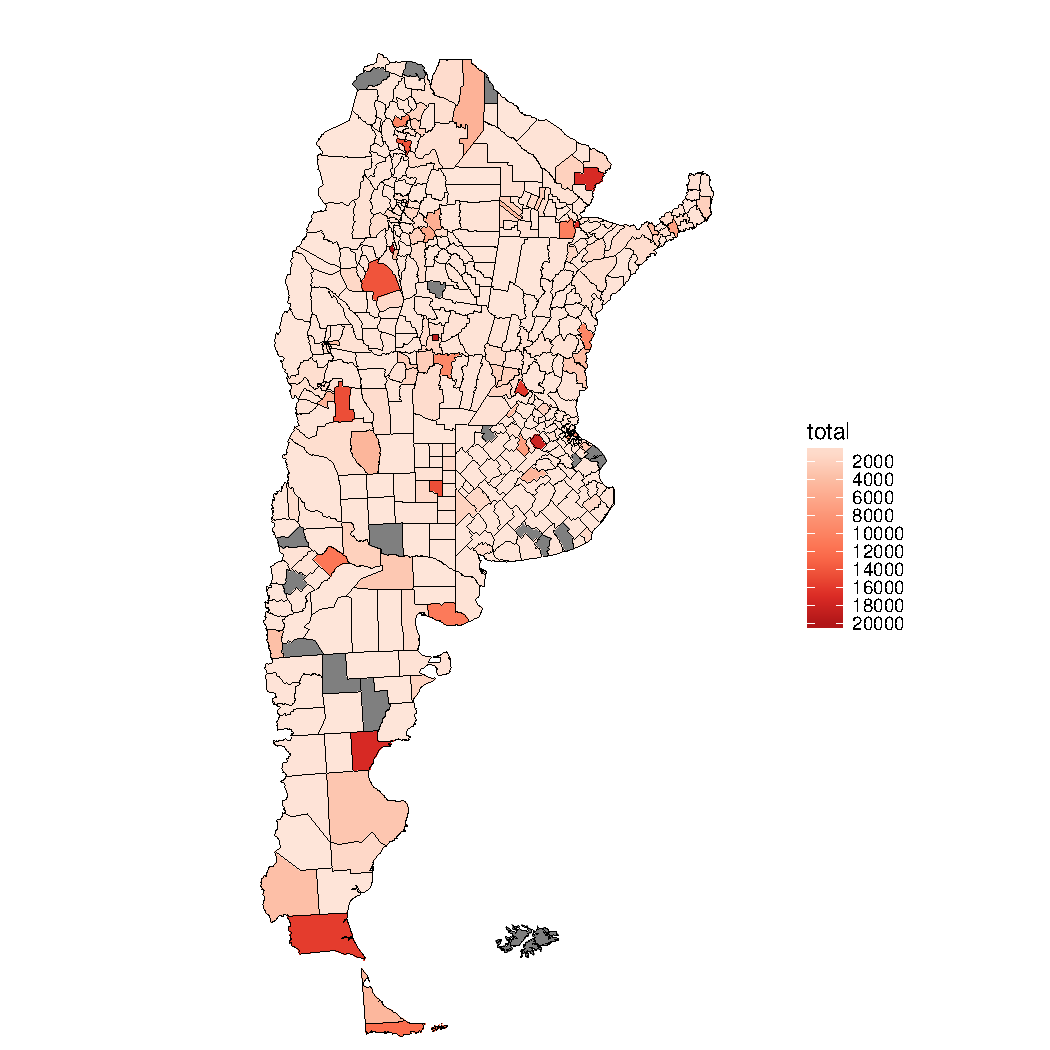
\includegraphics[width=1.0\textwidth]{./images/mapaGPS.pdf}
\caption{Mapa con la distribución de los tuits que incluyeron sus coordenadas geográficas. } 
\label{fig:mapaGPS} 
\end{figure}